\documentclass{presentation}

\title{The Role of Electronics Shops}
\subtitle{In a Research Environment}
\author{Blaise Thompson}

\institute{University of Wisconsin--Madison}
\date{2024-04-10}

\begin{document}
\maketitle

\section{Research Shops}

\begin{frame}\frametitle{UW-Madison Department of Chemistry}
  \huge
  What is a research electronics shop?
\end{frame}

\begin{frame}\frametitle{UW-Madison Department of Chemistry}
  \includegraphics[width=\textwidth]{"./staff.png"}
\end{frame}

\begin{frame}\frametitle{UW-Madison Department of Chemistry}
  three shops:
  \begin{itemize}
    \item machine
      \begin{itemize}
        \item three full time staff
        \item specialty focus on pump repair
      \end{itemize}
    \item glass
      \begin{itemize}
        \item two full time staff
      \end{itemize}
    \item electronics
      \begin{itemize}
        \item two full time staff
        \item four student workers
      \end{itemize}
  \end{itemize}
\end{frame}

\begin{frame}\frametitle{UW-Madison Department of Chemistry}
  Electronics at UW-Madison Chemistry
  \begin{itemize}
    \item here for as long as anyone can remember
      \begin{itemize}
        \item at least 50 years
      \end{itemize}
    \item historically much larger group
      \begin{itemize}
        \item more than seven full time staff, at peak
      \end{itemize}
    \item construct, repair, assist
  \end{itemize}
\end{frame}

{
\setbeamercolor{background canvas}{bg=selection}

\begin{frame}\frametitle{UW-Madison Department of Physics}
  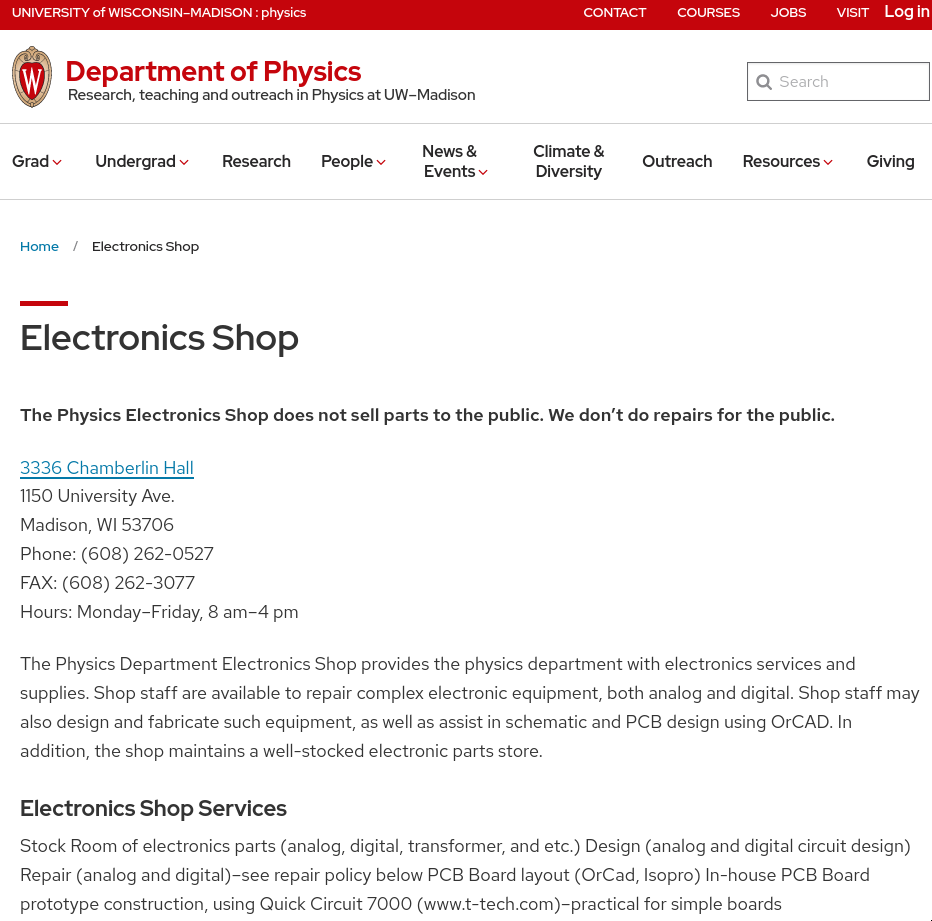
\includegraphics[width=\textwidth]{"./madison-physics.png"}
\end{frame}

\begin{frame}\frametitle{UW-Madison Physical Sciences Lab}
  
\includegraphics[width=\textwidth]{"./psl.png"}
\end{frame}

\begin{frame}\frametitle{Purdue Amy Facility}
  
\includegraphics[width=\textwidth]{"./amy.png"}
\end{frame}

\begin{frame}\frametitle{University of Washington}
  
\includegraphics[width=\textwidth]{"./washington.png"}
\end{frame}

\begin{frame}\frametitle{University of Colorado Boulder}
  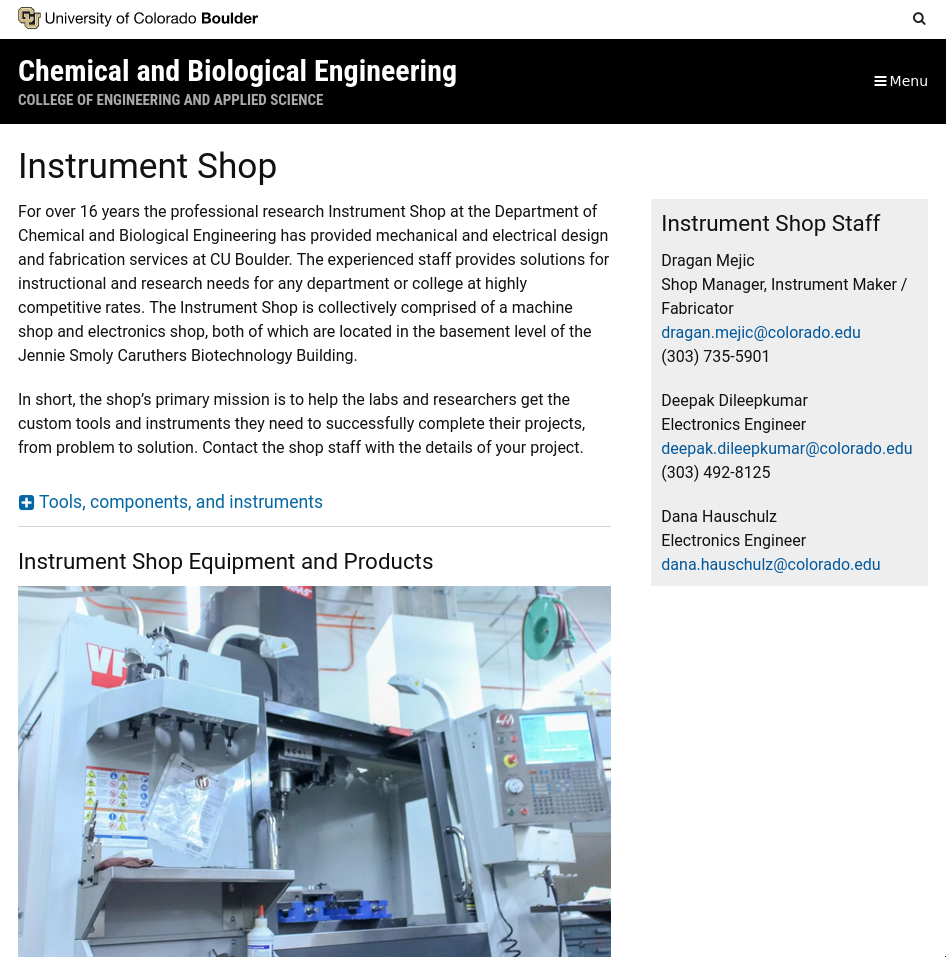
\includegraphics[width=\textwidth]{"./cu-boulder.png"}
\end{frame}

\begin{frame}\frametitle{University of Pittsburgh}
  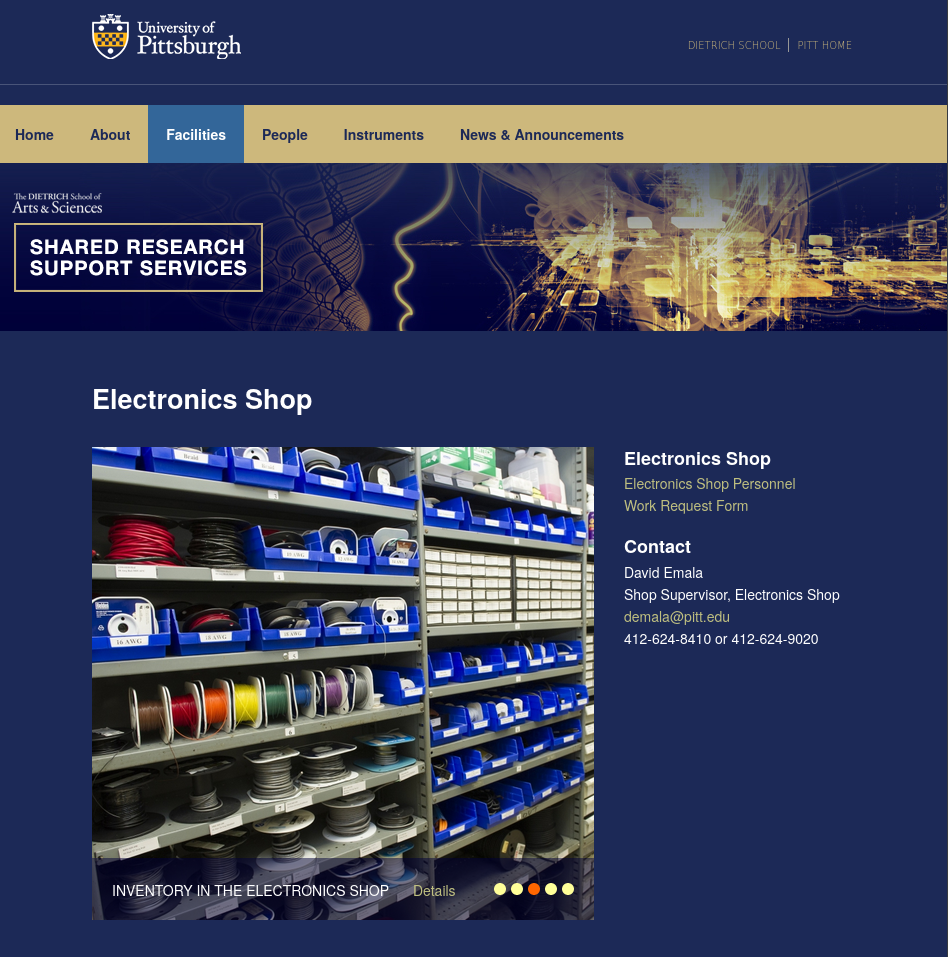
\includegraphics[width=\textwidth]{"./pittsburgh.png"}
\end{frame}

\begin{frame}\frametitle{Indiana University Bloomington}
  
\includegraphics[width=\textwidth]{"./bloom.png"}
\end{frame}

\begin{frame}\frametitle{UNC Chapel Hill}
  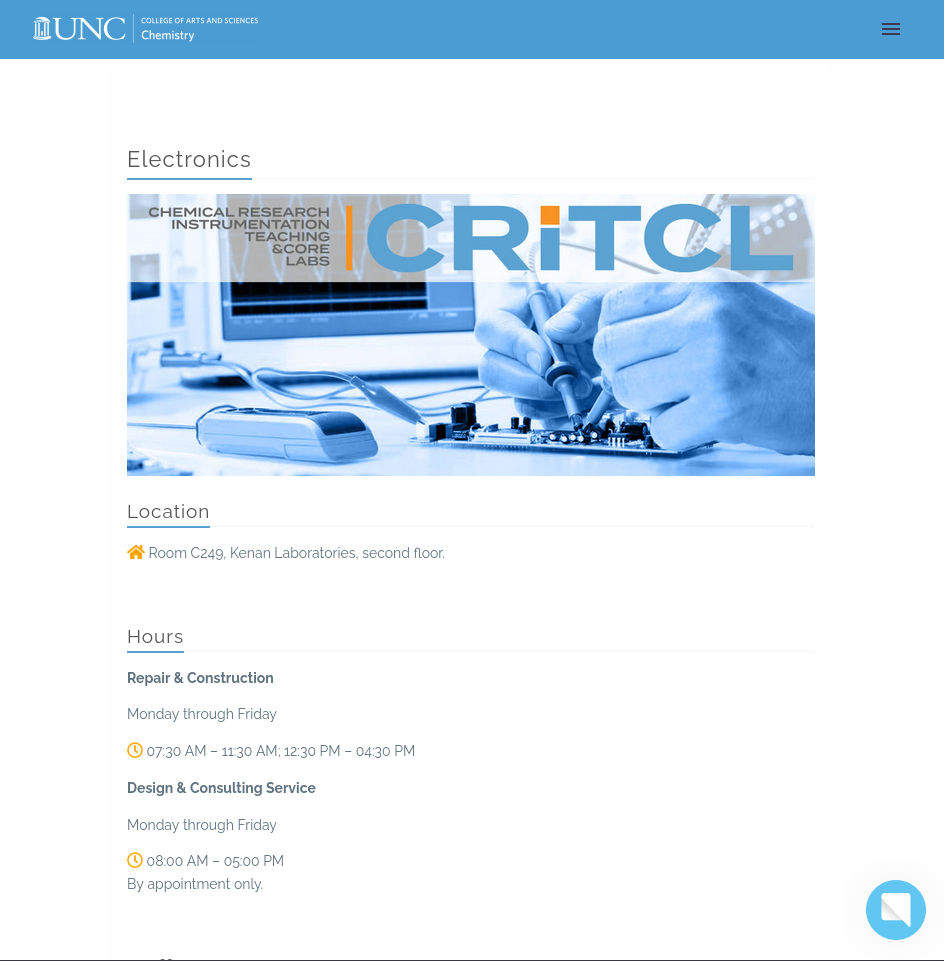
\includegraphics[width=\textwidth]{"./unc.png"}
\end{frame}

\begin{frame}\frametitle{Arizona State University}
  
\includegraphics[width=\textwidth]{"./asu.png"}
\end{frame}

\begin{frame}\frametitle{Stanford}
  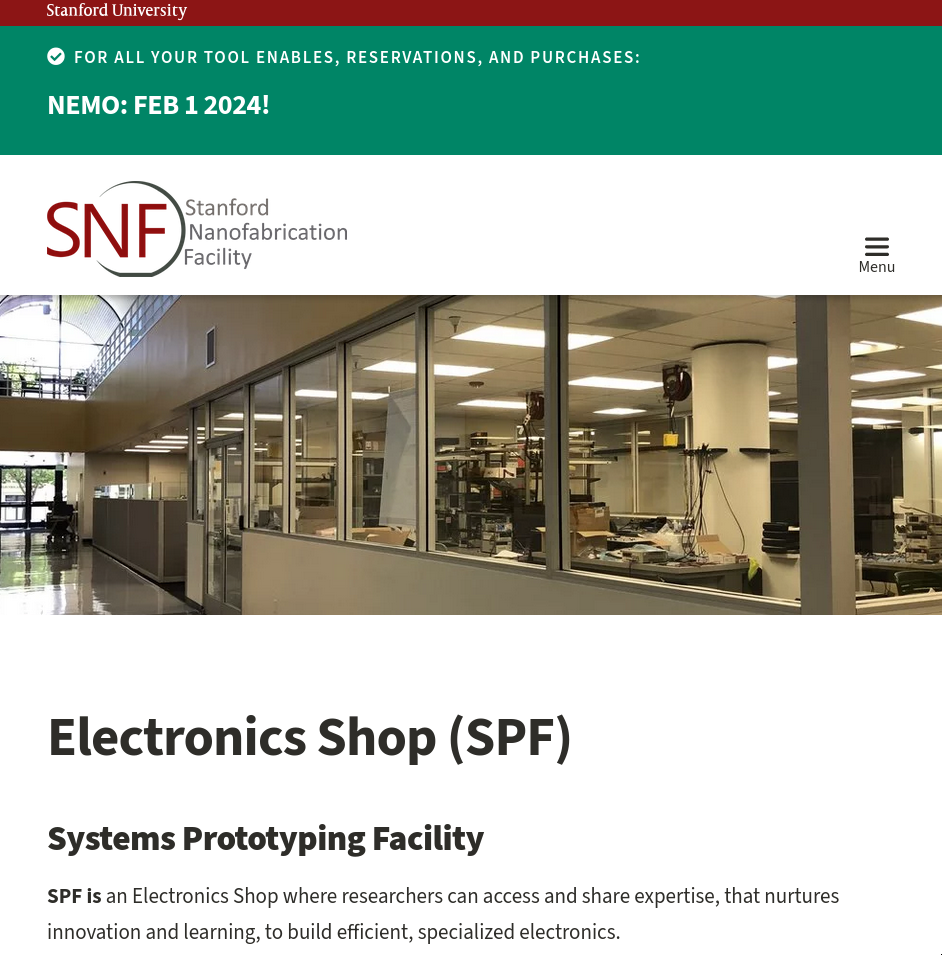
\includegraphics[width=\textwidth]{"./stanford.png"}
\end{frame}

\begin{frame}\frametitle{Brown}
  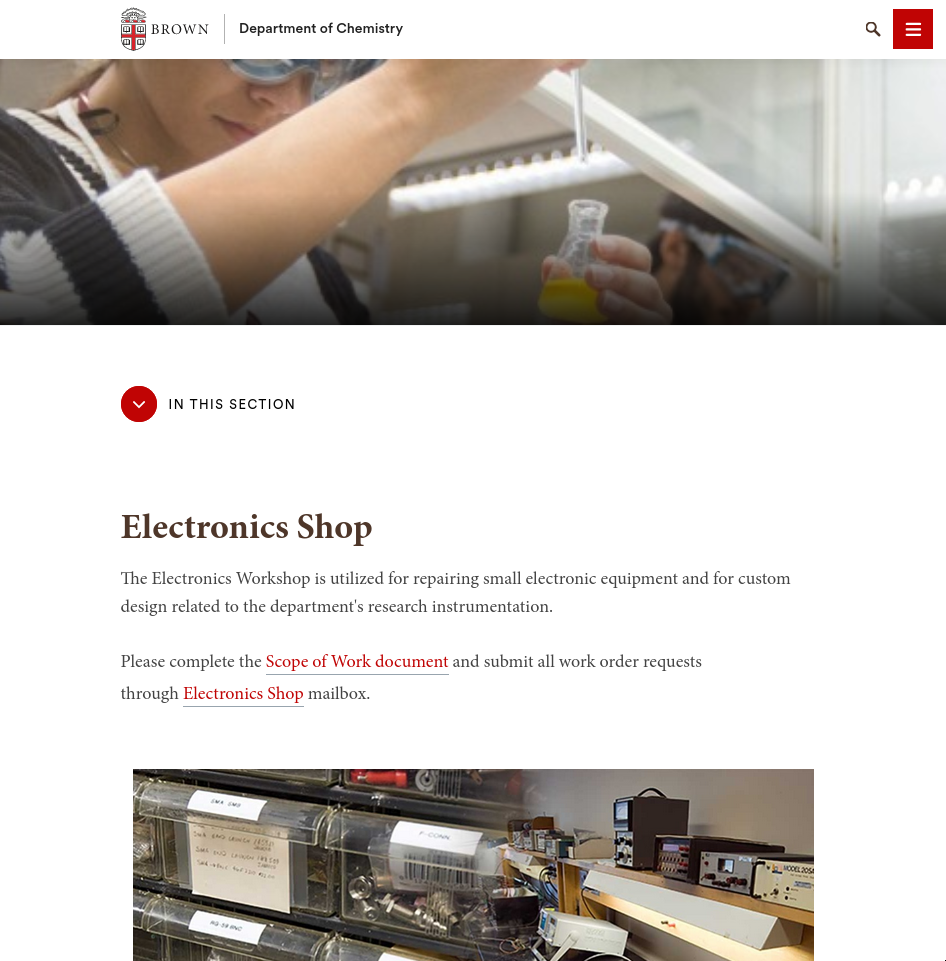
\includegraphics[width=\textwidth]{"./brown.png"}
\end{frame}

}

\section{Custom Research Electronics}

\begin{frame}
  \huge
  Custom electronics for research?
\end{frame}

\begin{frame}\frametitle{XyloTron}
  \fbox{
    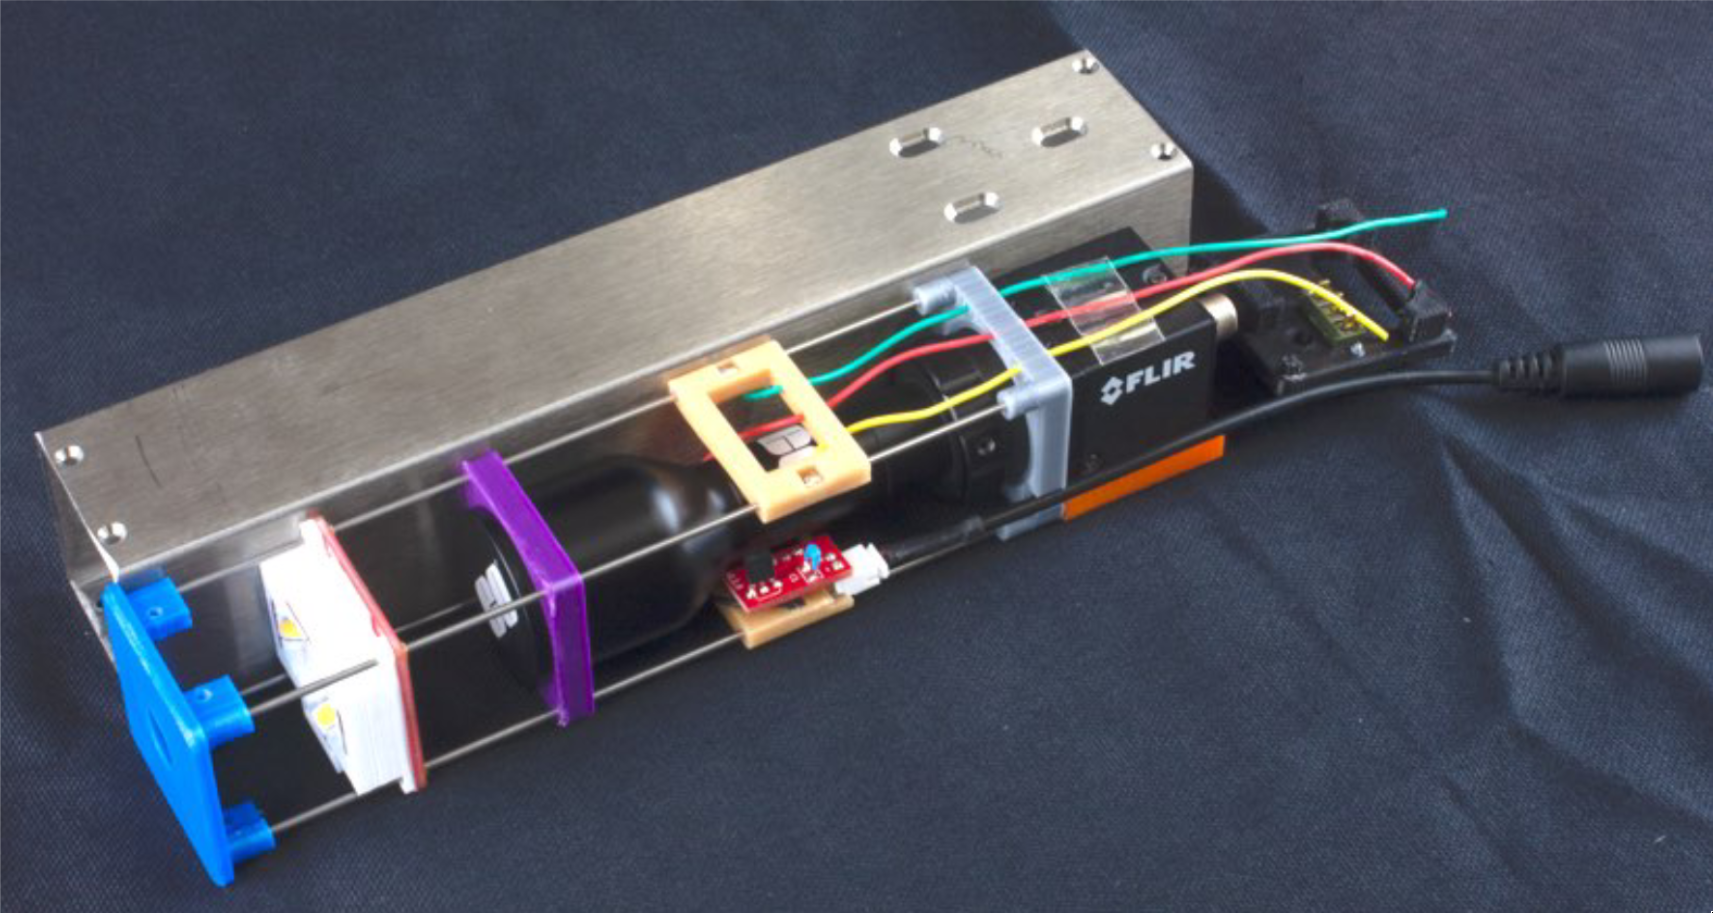
\includegraphics[width=\textwidth]{"./xylotron.pdf"}
  }
\end{frame}

\begin{frame}\frametitle{XyloTron}
  xylotron picture here please
\end{frame}

\begin{frame}\frametitle{Gas Uptake}
  \fbox{
    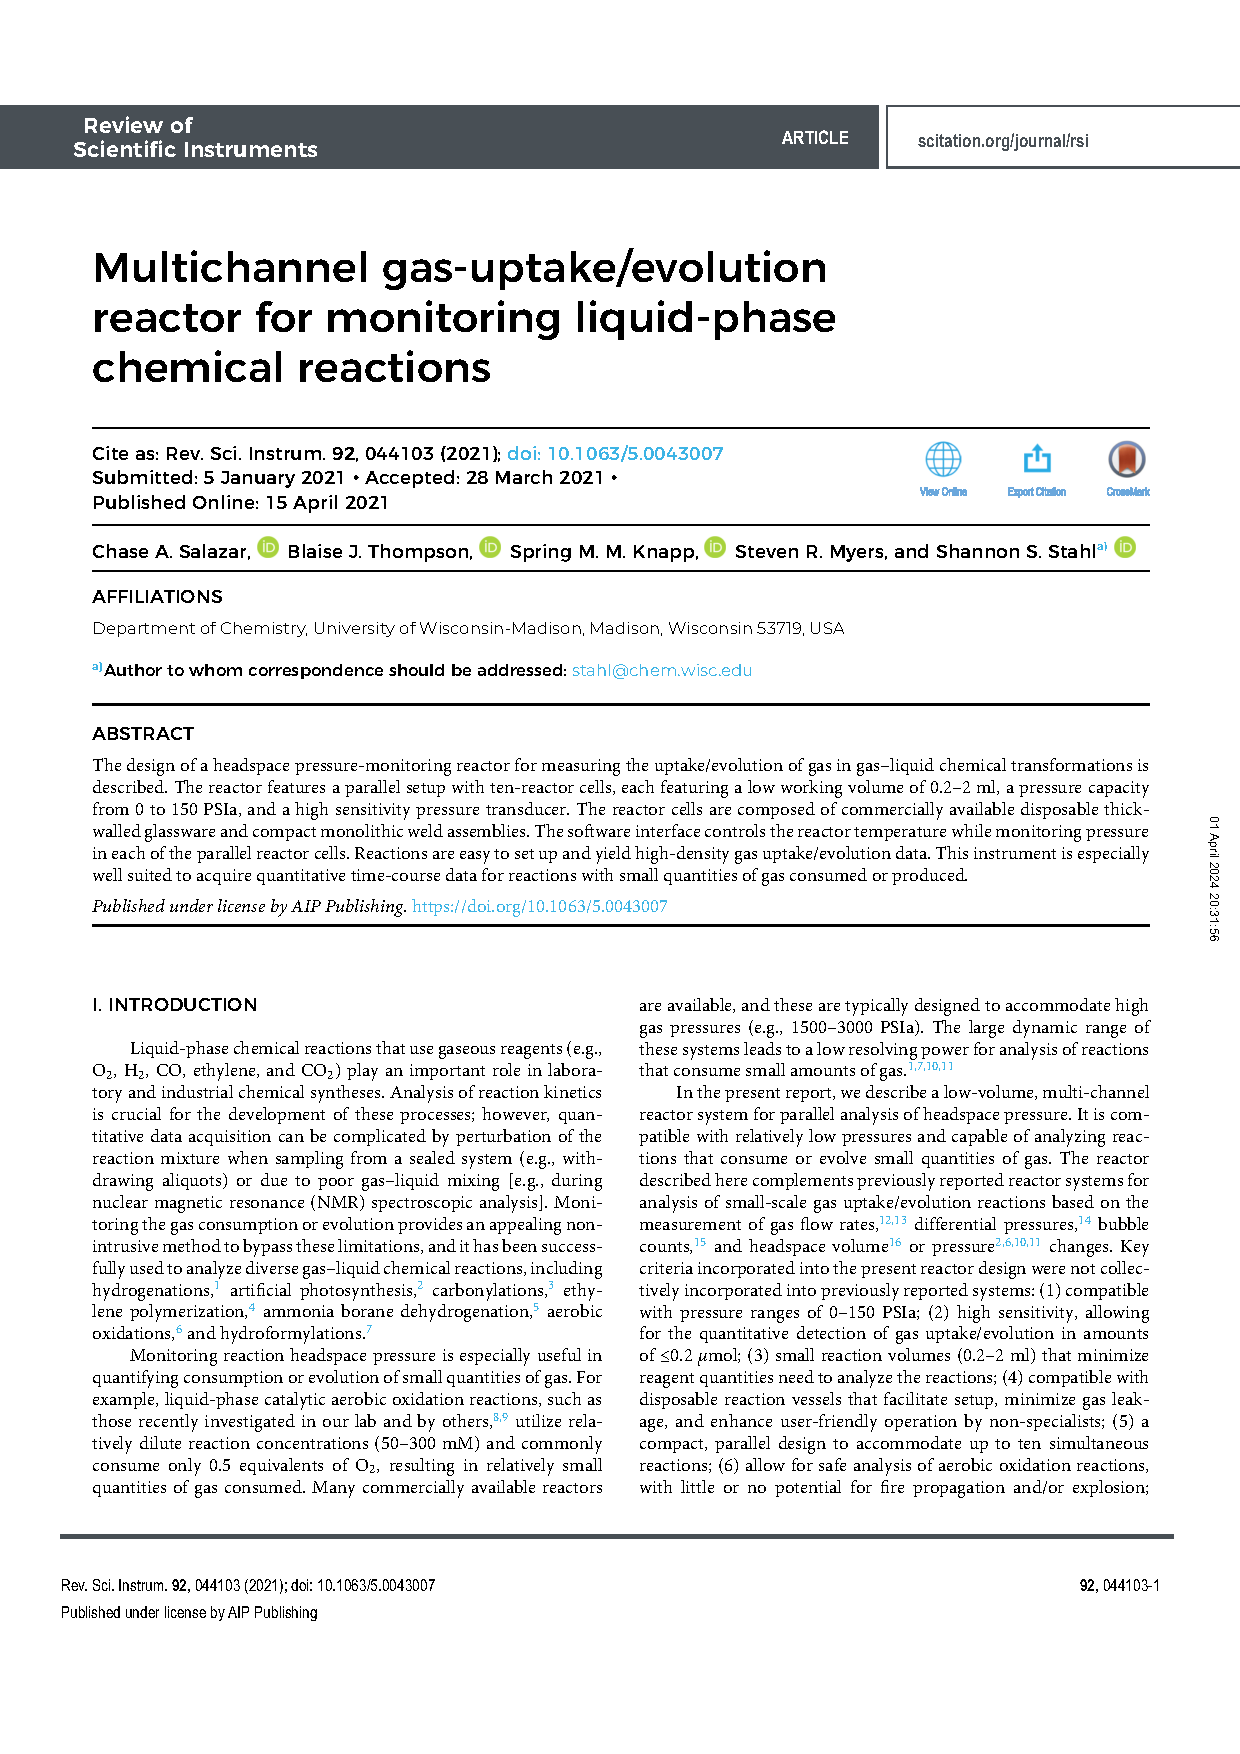
\includegraphics[width=\textwidth]{"./gas-uptake.pdf"}
  }
\end{frame}

\begin{frame}\frametitle{Gas Uptake}
  gas uptake picture here please
\end{frame}

\begin{frame}\frametitle{Photoreactor}
  \fbox{
    \includegraphics[width=\textwidth]{"./lampkin.pdf"}
  }
\end{frame}

\begin{frame}\frametitle{Photoreactor}
  photoreactor picture here please
\end{frame}


\begin{frame}\frametitle{Oscillator}
  \fbox{
    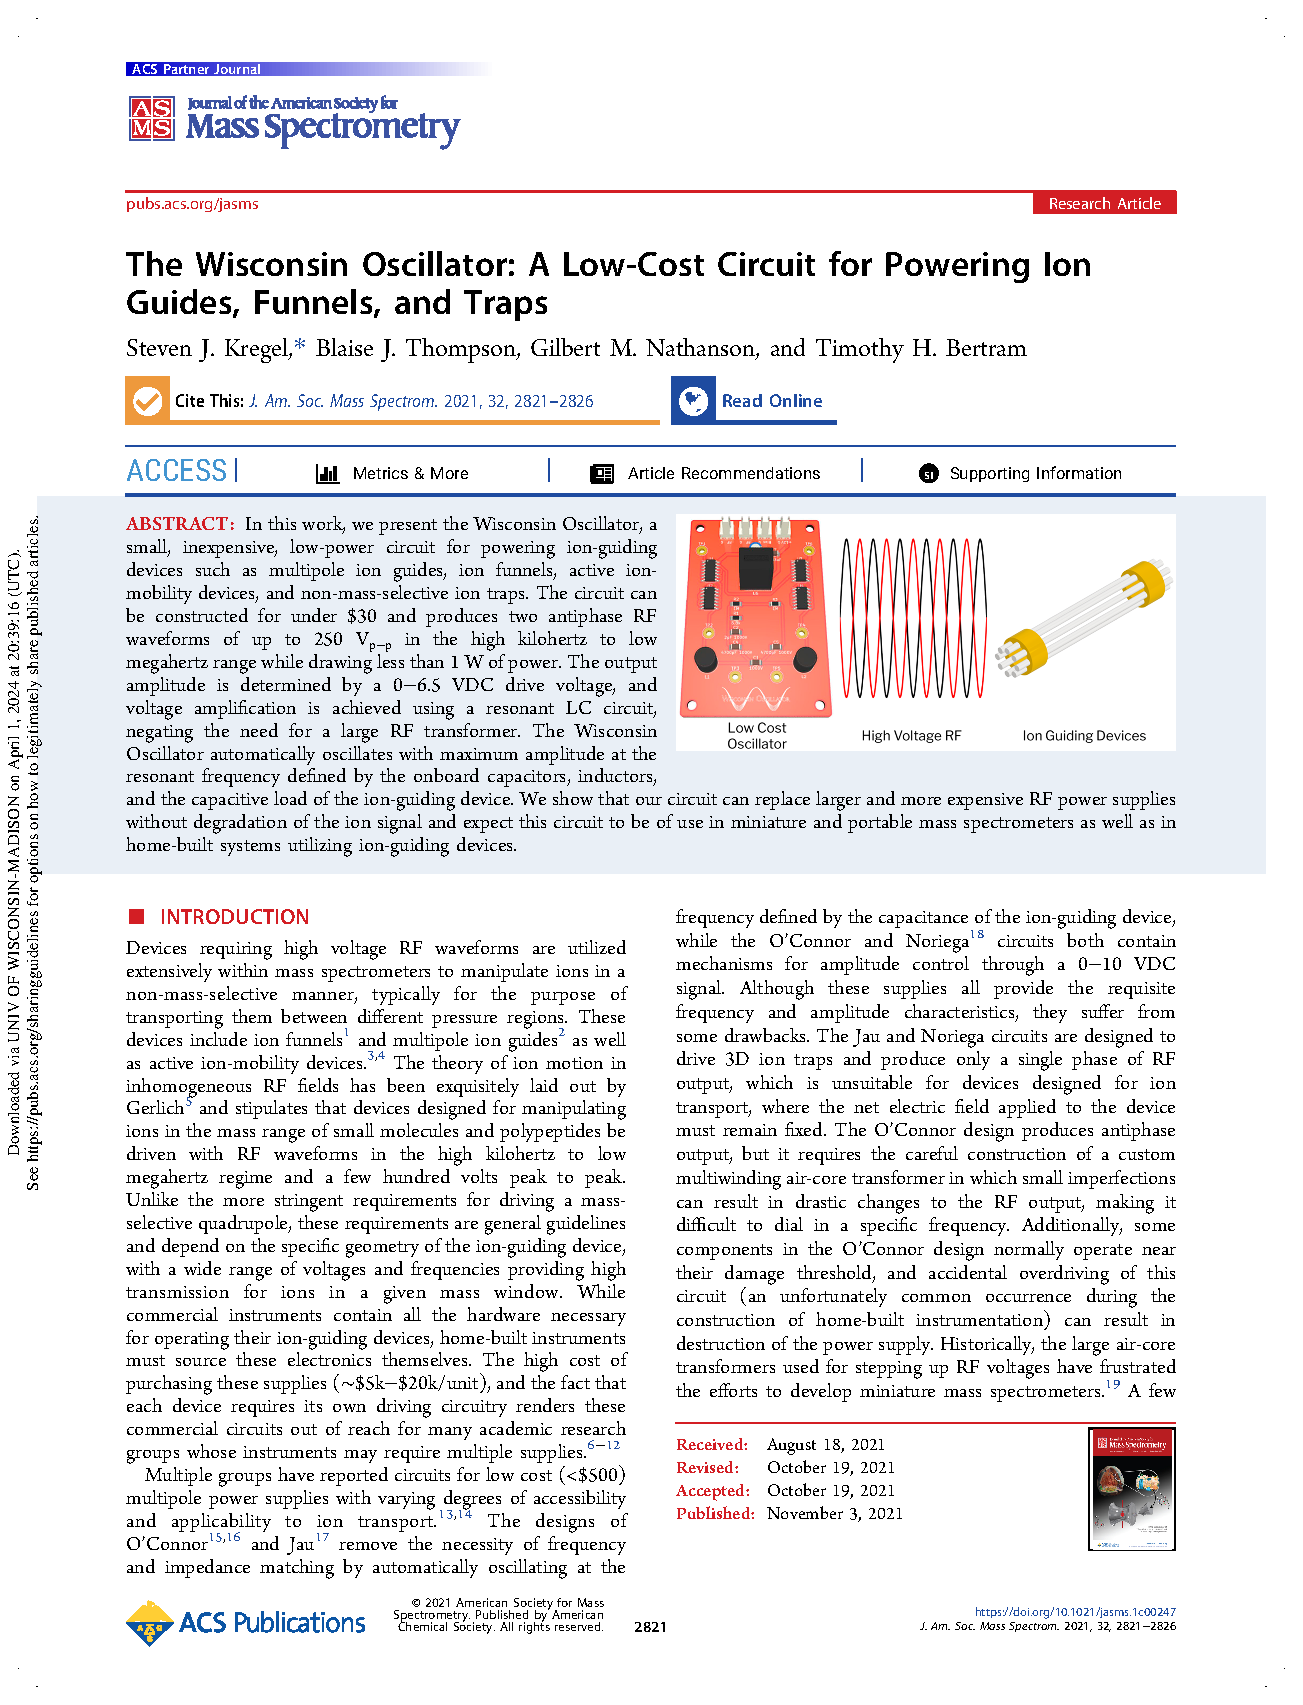
\includegraphics[width=\textwidth]{"./kregel.pdf"}
  }
\end{frame}

\begin{frame}\frametitle{Oscillator}
  oscillator picture here please
\end{frame}


\section{Instrument \& Appliance Maintenance}

\begin{frame}
  \huge
  Repair and maintenance of research equipment.
\end{frame}

\begin{frame}\frametitle{Amber Bartz}
  \begin{columns}
    \begin{column}{0.33\textwidth}
      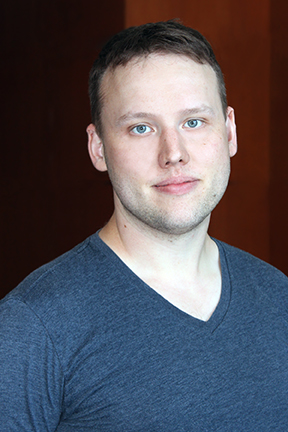
\includegraphics[width=\textwidth]{"./Thompson_Blaise_LowRes.jpg"}
    \end{column}
    \begin{column}{0.67\textwidth}
      Amber Bartz \\
      Chemistry Electronics Shop \\
      afbartz@wisc.edu
      \vskip 3 em
      Check out Amber's poster presentation: \\
      \emph{What Researchers Should Know When Powering Lab Equipment}
    \end{column}
  \end{columns}
\end{frame}


\section{Electrical Safety}

\begin{frame}\frametitle{Humility}
  Shop staff are not safety experts.
  \vfill
  Thank YOU ALL.
\end{frame}

\section{Thank You}

\begin{frame}\frametitle{Thank You}
  \begin{columns}
    \begin{column}{0.33\textwidth}
      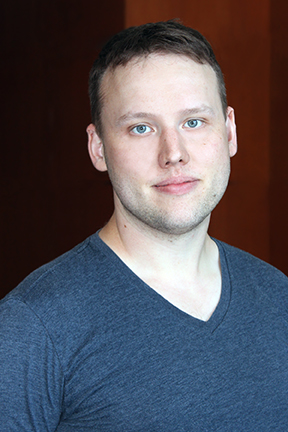
\includegraphics[width=\textwidth]{"./Thompson_Blaise_LowRes.jpg"}
    \end{column}
    \begin{column}{0.67\textwidth}
      Blaise Thompson \\
      Chemistry Electronics Shop \\
      blaise.thompson@wisc.edu
      \vskip 3 em
      We are here to help you use electrical equipment in your research.
      Please reach out!
      \vskip 3 em
      \hl{Questions?}
    \end{column}
  \end{columns}
\end{frame}

\end{document}
